% Lookback Validity Audit — NEMI 2026 poster, v1
% 3-column, 3-row. Same style as mechviews/RTI posters.
%
%   cd poster && lualatex lookback_poster_v1.tex

\documentclass[28pt, a0paper, portrait]{tikzposter}

\usepackage{amsmath,amssymb}
\usepackage{array}
\usepackage{booktabs}
\usepackage{graphicx}
\usepackage{enumitem}
\usepackage{microtype}

\graphicspath{{../paper/figures/}{figures/}}

% ── Color palette ───────────────────────────────────────
\definecolor{darktext}{HTML}{2C3E50}
\definecolor{blockbg}{HTML}{FFFFFF}
\definecolor{auditblue}{HTML}{2980B9}
\definecolor{resultgreen}{HTML}{27AE60}
\definecolor{surprisered}{HTML}{E74C3C}
\definecolor{verdictpurple}{HTML}{8E44AD}
\definecolor{qwenorange}{HTML}{E67E22}

% ── Theme ───────────────────────────────────────────────
\usetheme{Default}

\definecolorstyle{AuditColors}{
  \definecolor{colorOne}{HTML}{2C3E50}
  \definecolor{colorTwo}{HTML}{3498DB}
  \definecolor{colorThree}{HTML}{ECF0F1}
}{
  \colorlet{backgroundcolor}{colorThree}
  \colorlet{framecolor}{colorOne}
  \colorlet{titlefgcolor}{white}
  \colorlet{titlebgcolor}{colorOne}
  \colorlet{blocktitlebgcolor}{colorTwo}
  \colorlet{blocktitlefgcolor}{white}
  \colorlet{blockbodybgcolor}{blockbg}
  \colorlet{blockbodyfgcolor}{darktext}
  \colorlet{notefgcolor}{darktext}
  \colorlet{notebgcolor}{auditblue!12}
  \colorlet{notefrcolor}{auditblue}
}
\usecolorstyle{AuditColors}

\defineblockstyle{AuditBlock}{
  titlewidthscale=1.0, bodywidthscale=1.0, titleleft,
  titleoffsetx=0pt, titleoffsety=0pt,
  bodyoffsetx=0pt, bodyoffsety=0pt, bodyverticalshift=0pt,
  roundedcorners=12, linewidth=2pt, titleinnersep=10pt, bodyinnersep=12pt
}{
  \draw[rounded corners=\blockroundedcorners, color=blocktitlebgcolor,
        fill=blockbodybgcolor, line width=\blocklinewidth]
    (blockbody.south west) rectangle (blocktitle.north east);
  \ifBlockHasTitle
    \draw[rounded corners=\blockroundedcorners,
          fill=blocktitlebgcolor, color=blocktitlebgcolor,
          line width=\blocklinewidth]
      (blocktitle.south west) rectangle (blocktitle.north east);
  \fi
}
\useblockstyle{AuditBlock}

\definetitlestyle{AuditTitle}{
  width=\paperwidth, roundedcorners=0, linewidth=0pt, innersep=20pt,
  titletotopverticalspace=12mm, titletoblockverticalspace=20mm
}{
  \draw[fill=titlebgcolor, color=titlebgcolor]
    (\titleposleft, \titleposbottom)
    rectangle (\titleposright, \titlepostop);
}
\usetitlestyle{AuditTitle}

\title{%
  \parbox{0.92\linewidth}{\centering\bfseries
    Belief Tracking or Attention-Mediated Retrieval?\\[6pt]
    A Validity Audit of the Lookback Mechanism}}
\author{Elliot Tower\quad\texttt{elliot@elliottower.ai}}
\institute{}

\begin{document}

\maketitle[width=\paperwidth]

% ════════════════════════════════════════════════════════
% ROW 1
% ════════════════════════════════════════════════════════
\begin{columns}
\column{0.33}

{
\colorlet{blocktitlebgcolor}{auditblue}
\block{The Claim Under Audit}{
  Prakash et al.\ (ICLR 2026) report that Llama-3-70B tracks
  character beliefs via ``pointer dereference through attention''
  --- three sub-mechanisms at non-overlapping layer ranges.

  \begin{itemize}[leftmargin=*, itemsep=3mm]
    \item \textbf{Binding} (L33--38): links characters to containers
    \item \textbf{Answer} (L52--56): retrieves the believed content
    \item \textbf{Visibility} (L10--31): gates by observability
  \end{itemize}

  \vspace{4mm}
  We apply 35 validity criteria and find \textbf{6 untested
  assumptions}. Most critically: the evaluation never tests
  \textbf{false beliefs} --- belief equals reality in every
  story pair.
}
}

\column{0.34}

{
\colorlet{blocktitlebgcolor}{auditblue}
\block{Six Gaps}{
  \begin{itemize}[leftmargin=*, itemsep=3mm]
    \item \textbf{No random-subspace baseline} --- does a random
      subspace of matched rank achieve comparable IIA?
    \item \textbf{No negative controls} --- does the pattern appear
      on non-belief tasks?
    \item \textbf{No false beliefs} --- belief = reality in every
      pair by construction
    \item \textbf{No cross-stage test} --- are the three
      sub-mechanisms one causal chain or three separate processes?
    \item \textbf{Referential inflation} --- ``pointer dereference''
      redescribes what attention does by construction
    \item \textbf{No framing variation} --- only one question type
      tested
  \end{itemize}
}
}

\column{0.33}

{
\colorlet{blocktitlebgcolor}{resultgreen}
\block{The Subspaces Are Real}{
  \begin{itemize}[leftmargin=*, itemsep=3mm]
    \item Beat random subspaces at all layers ($p = 0.005$,
      rank test, $n = 200$)
    \item Beat shuffled-label controls ($p < 0.05$ for 4 of 6
      subspaces)
    \item Replicate on Llama-3.1 within $\pm 0.05$ at binding
      layers; answer layers reach \textbf{ceiling}
    \item Transfer across story templates (L38 IIA $= 0.957$)
    \item 19/20 positive effects robust to unmeasured confounding
      ($E \geq 2.0$)
  \end{itemize}
}
}

\end{columns}

% ════════════════════════════════════════════════════════
% ROW 2
% ════════════════════════════════════════════════════════
\begin{columns}
\column{0.33}

{
\colorlet{blocktitlebgcolor}{surprisered}
\block{The Decisive Result: Framing Dissociation}{
  Same story pairs, same underlying fact, four question framings:

  \vspace{4mm}
  \begin{center}
  \renewcommand{\arraystretch}{1.4}
  {\large
  \begin{tabular}{@{}lccc@{}}
    \toprule
    \textbf{Framing} & \textbf{L38} & \textbf{L52} & \textbf{L53} \\
    \midrule
    ``What does X believe\ldots'' & \textbf{1.00} & \textbf{1.00} & \textbf{1.00} \\
    ``What did X put\ldots'' & .89 & .40 & .06 \\
    ``What is inside\ldots'' & .00 & .00 & .00 \\
    ``X filled\ldots with'' & .00 & .00 & .00 \\
    \bottomrule
  \end{tabular}}
  \end{center}

  \vspace{4mm}
  Which drink is in which container is \textbf{identical} across
  all four framings. The subspace responds to the
  \textbf{epistemic framing}, not the fact.

  \vspace{4mm}
  If the subspaces encoded generic entity-state bindings,
  reality-state questions would transfer. They do not.
}
}

\column{0.34}

{
\colorlet{blocktitlebgcolor}{surprisered}
\block{Three Predictions Overturned}{
  We predicted the subspaces would encode generic entity-state
  bindings. Three experiments overturned this --- each time
  \textbf{strengthening} the original claim.

  \vspace{4mm}
  \textbf{False beliefs} ($n = 80$, 100\% behavioral accuracy)

  Character places a drink; another swaps it unobserved.
  We predicted IIA $< 0.30$.
  Result: L38 = \textbf{0.975}, L52 = \textbf{0.975}.

  \vspace{4mm}
  \textbf{Observed knowledge} ($n = 80$, 88\% accuracy)

  Character observes another's action; question asks what
  the observer knows. We predicted IIA $< 0.30$.
  Result: L38 = \textbf{0.988}, L52 = \textbf{0.975}.

  \vspace{4mm}
  \textbf{Framing dissociation} ($n = 35$)

  We predicted IIA within $\pm 0.10$ across framings.
  Result: belief = 1.0, reality = \textbf{0.0}.
}
}

\column{0.33}

{
\colorlet{blocktitlebgcolor}{qwenorange}
\block{Cross-Model: Partial Transfer}{
  We apply the mismatch test to \textbf{Qwen2.5-14B} ($n = 200$).

  \vspace{4mm}
  \textbf{Answer lookback transfers:}
  \begin{itemize}[leftmargin=*, itemsep=2mm]
    \item Recalled-only IIA = 0.005
    \item Lookback-only IIA = 0.000
    \item Both IIA = \textbf{1.000}
    \item Singles near zero, pair at ceiling --- same
      dependency structure as Llama
  \end{itemize}

  \vspace{4mm}
  \textbf{Binding does not transfer:}
  \begin{itemize}[leftmargin=*, itemsep=2mm]
    \item Recalled-only IIA = 1.0 at all layers
    \item Combined patch yields IIA = \textbf{0.0}
    \item Structurally different from Llama --- full-residual
      patching cannot detect this
  \end{itemize}

  \vspace{4mm}
  ``Same underlying mechanism'' is accurate for answer lookback
  and false for binding.
}
}

\end{columns}

% ════════════════════════════════════════════════════════
% ROW 3
% ════════════════════════════════════════════════════════
\begin{columns}
\column{0.33}

\block{IIA Across All Experiments}{
  \begin{center}
  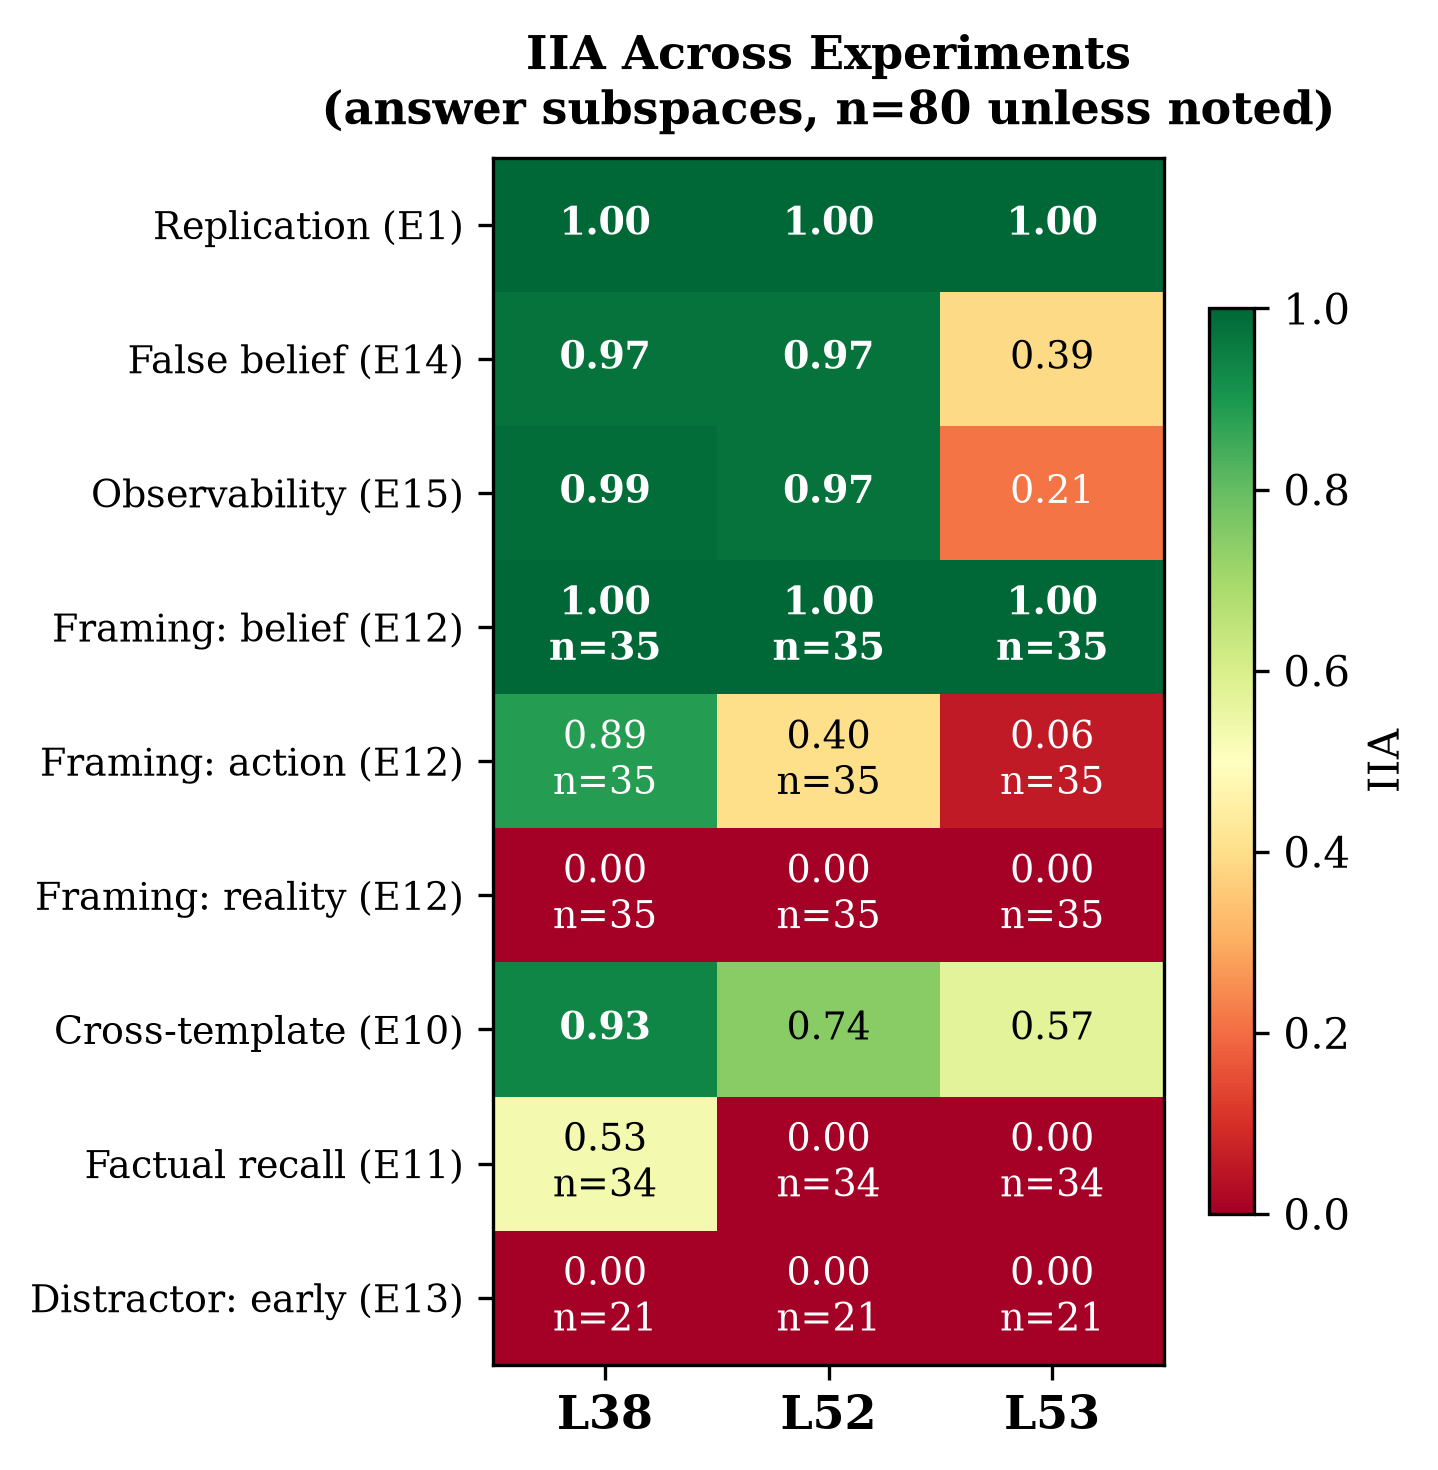
\includegraphics[width=0.95\linewidth]{fig1_iia_heatmap.pdf}
  \end{center}

  \vspace{2mm}
  L38 and L52 achieve near-ceiling IIA on belief tasks and zero
  on perspective-free queries. L53 is unreliable (high seed
  variance, $p = 0.286$ vs.\ shuffled labels).
}

\column{0.34}

{
\colorlet{blocktitlebgcolor}{verdictpurple}
\block{Verdict: Causally Suggestive $\to$ Mechanistically Supported}{
  The subspaces encode character-state associations that:
  \begin{itemize}[leftmargin=*, itemsep=3mm]
    \item Update with observability and state changes
    \item Track beliefs that diverge from reality
    \item Respond specifically to character-perspective queries
    \item Are absent on perspective-free questions about the same
      facts
  \end{itemize}

  \vspace{4mm}
  This is richer than ``retrieval'' but more precise than
  ``belief tracking.'' We propose \textbf{belief-constitutive
  entity binding}: the entity bindings constitute beliefs in
  the functional sense.

  \vspace{4mm}
  \textbf{Gap to Triangulated:} convergent evidence from an
  independent method (weight analysis, probing) and
  multi-seed cross-model replication.
}
}

\column{0.33}

{
\colorlet{blocktitlebgcolor}{colorOne}
\block{Takeaway}{
  {\Large\bfseries We designed experiments to find entity
  binding and found belief tracking instead.}

  \vspace{5mm}
  \begin{itemize}[leftmargin=*, itemsep=3mm]
    \item \textbf{35} validity criteria applied, \textbf{6} gaps
      identified
    \item \textbf{9} experiments completed on Llama-3.1-70B
    \item \textbf{3/4} dissociation predictions overturned ---
      each strengthening the claim
    \item Framing dissociation: IIA = 1.0 (belief) vs.\ 0.0
      (reality) on identical facts
    \item Cross-model: answer lookback transfers to Qwen,
      binding does not
  \end{itemize}

  \vspace{6mm}
  \begin{center}
  \texttt{elliot@elliottower.ai}

  \vspace{3mm}
  {\small All experiments, amendments, and code:}

  \texttt{github.com/elliottower/lookback-validity-audit}
  \end{center}
}
}

\end{columns}

\end{document}
